\documentclass[thesis]{subfiles}

\begin{document}

\chapter{Testy}

Niniejszy rozdział opisuje przeprowadzone testy funkcjonalne części serwerowej i~klienckiej stworzonej aplikacji.

%------------------------------------------------------------------------------
%
%\section{Monitorowanie wykorzystania zasobów}
%
%\noindent Poniżej przedstawiono testy użycia zasobów, takich jak:\mynobreakpar
%\begin{itemize}
%	\item pamięci,
%	\item plików,
%	\item \glslink{socket}{socketów},
%	\item \gls{fifo} (potok nazwany).
%\end{itemize}
%
%------------------------------------------------------------------------------

\section{Testy funkcjonalne}

Przeprowadzone testy wykonano w~środowisku złożonym z~trzech fizycznych komputerów klasy~PC oraz~dwóch maszyn wirtualnych \hrefemph{https://www.virtualbox.org/}{VirtualBox~5.1}. Wszystkie te~komputery miały zainstalowanym systemem \emph{Linux Debian}. Jeden z~fizycznych komputerów odgrywał jednocześnie rolę serwera i~klienta, a~pozostałe komputery są~klientami. Schemat testowej sieci został przedstawiony na rysunku~\ref{fig:testing-network}.

\begin{figure}
	\centering
	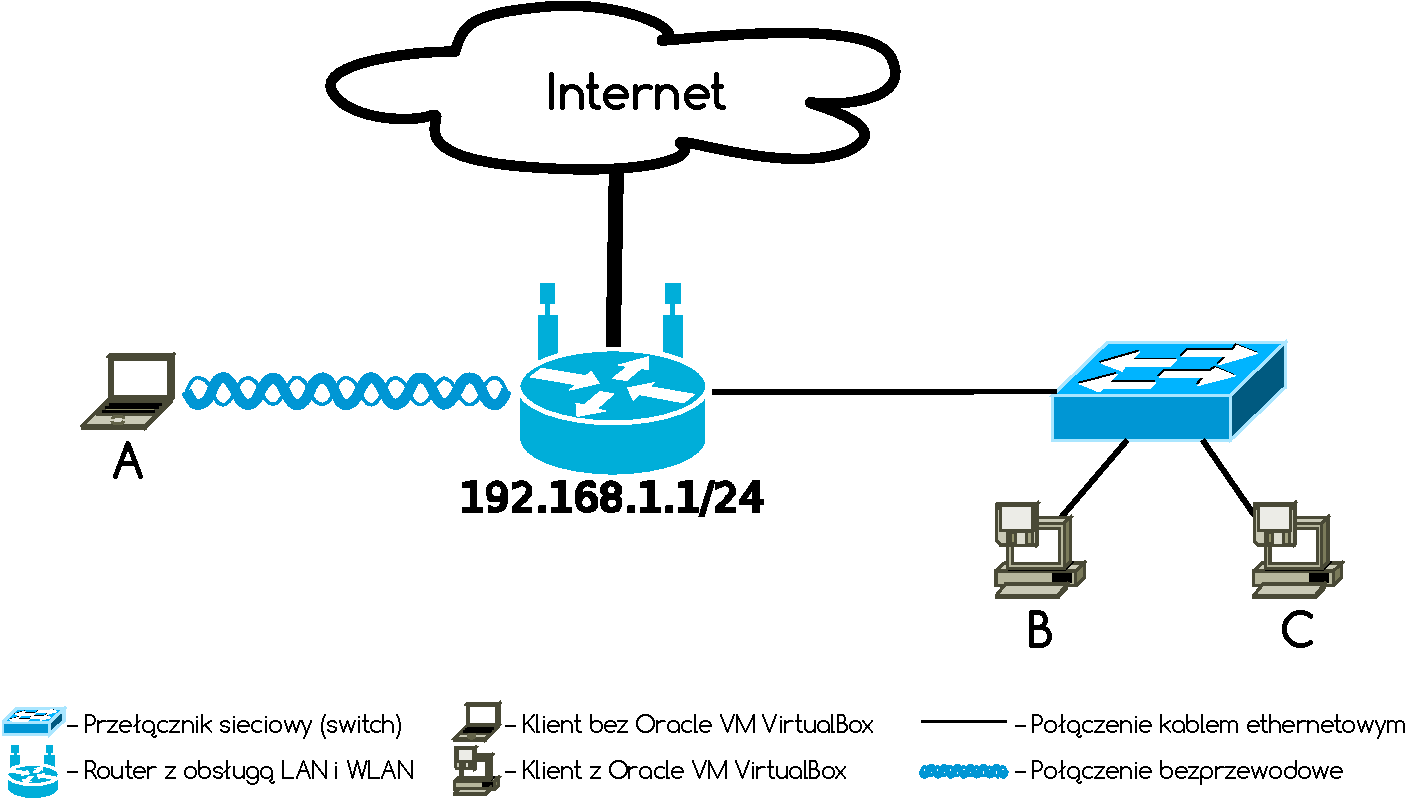
\includegraphics[width=0.85\textwidth]{img/testing-network}
	\caption{Schemat przedstawiający konfigurację sieciową użytego środowiska testowego}
	\label{fig:testing-network}
\end{figure}

TODO

\end{document}
